\documentclass[titlepage,landscape]{seminar}
\usepackage{url}
\usepackage{graphicx}
\usepackage{hyperref}
\usepackage{epstopdf}
\usepackage{slides}

\newcommand{\frack}{\frac{1}{k}}
\newcommand{\quarter}{\frac{1}{4}}

\begin{document}

\myslide{
  \heading{High-throughput sequencing}

  \begin{itemize}

  \item RAD-seq

  \item GBS - genotyping by sequencing

  \item WGS - whole-genome sequencing

  \end{itemize}
}

\myslide{
  \heading{{\it Wyeomyia smithii\/} ({\it COI\/})}

  \begin{itemize}

  \item 1176 bp segment

  \item 20 populations of {\it W. smithii}

    \item One population each of {\it W. mitchellii\/} and {\it
        W. vanduzeei\/} (as outgroups)

  \end{itemize}
}

\myslide{
\heading{{\it Wyeomyia smithii\/} ({\it COI\/})}
\begin{center}
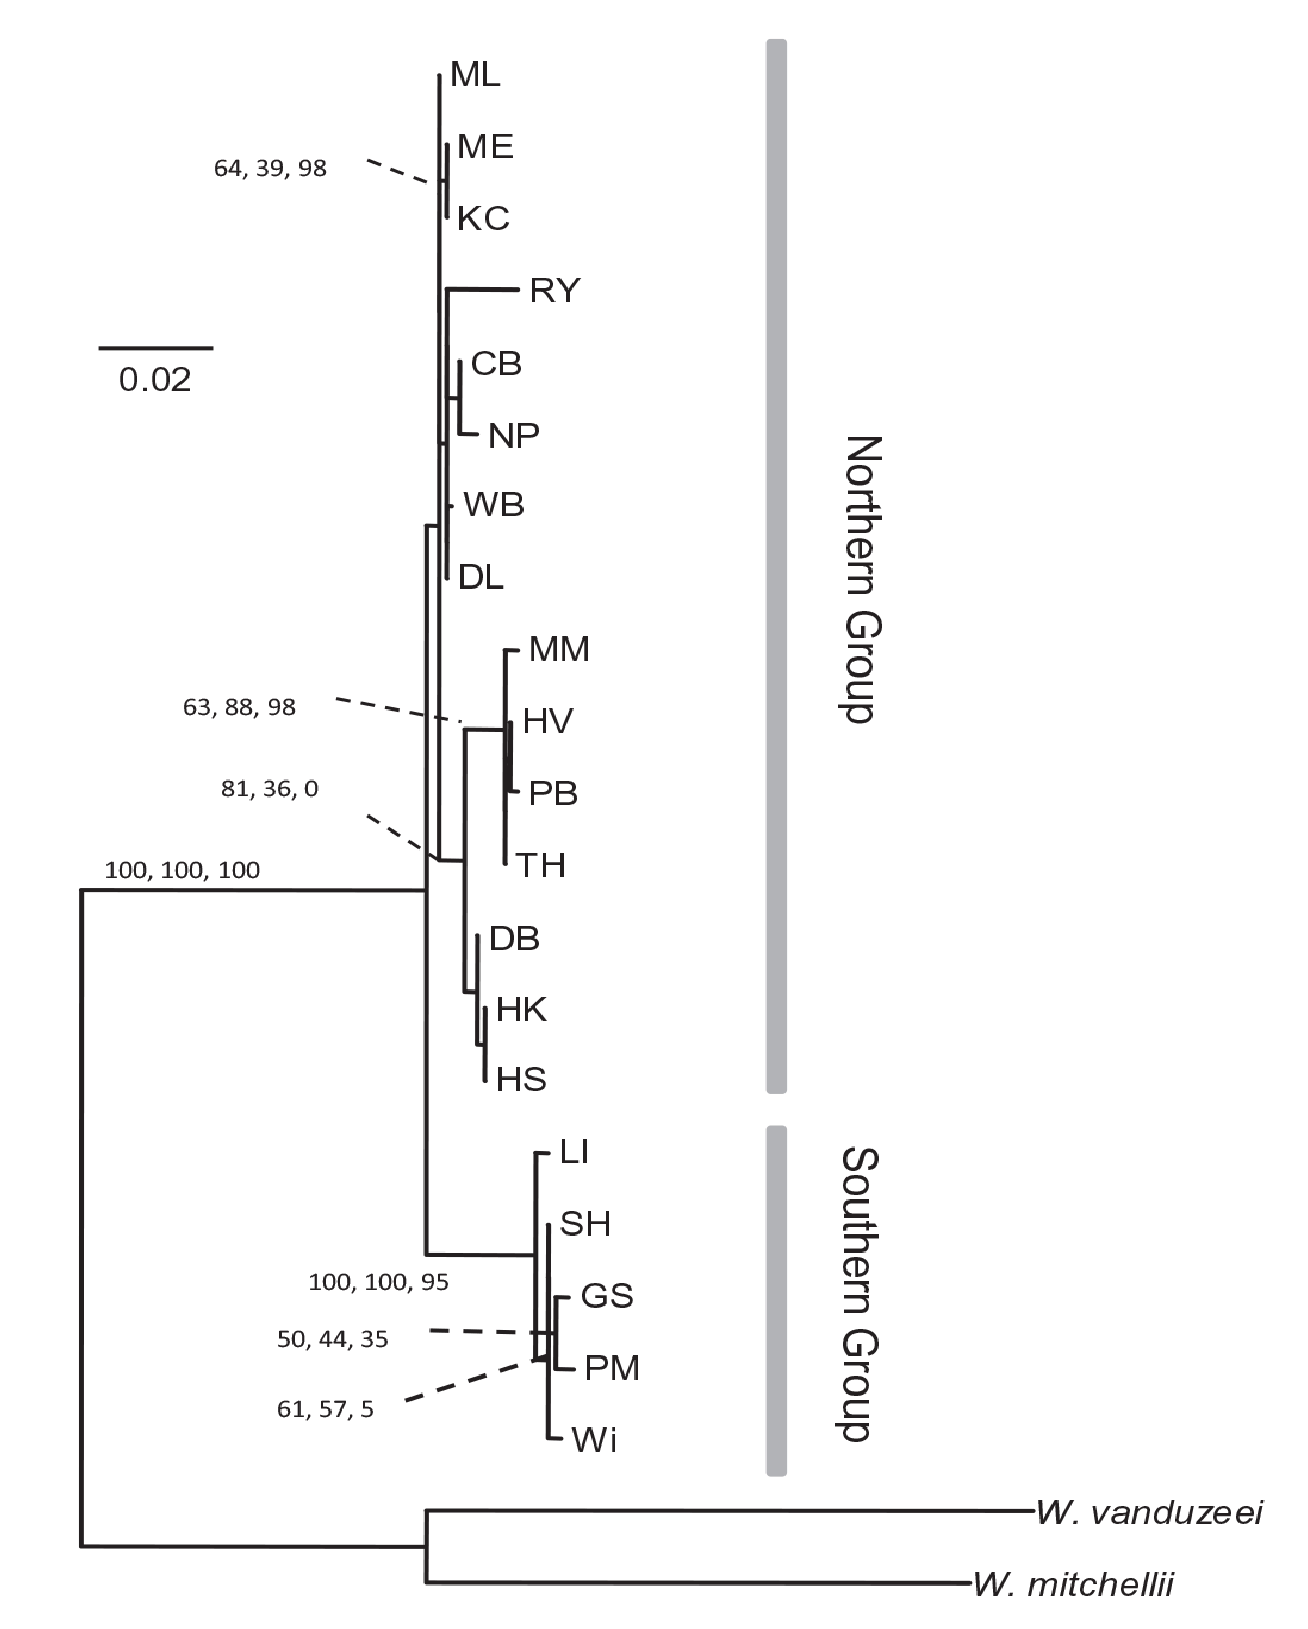
\includegraphics[height=0.9\textheight]{wyeomyia-COI.eps}
\end{center}
}

\myslide{
\heading{{\it Wyeomyia smithii\/} (RAD-seq)}
\begin{center}
\includegraphics[height=0.9\textheight]{RAD-tag.eps}
\end{center}
}

\myslide{
  \heading{{\it Wyeomyia smithii\/} (RAD-seq)}

  \begin{itemize}

   \item 21 populations, pooled sample of six individuals in each
     population, diegested with SbfI (CCTGCA$|$GG)

   \item 27.5M sequences, 14.9M passed quality control, each
     population rerpesented by $711,702 \pm 85,779$ sequences.

   \item $20,868 \pm 1681$ stacks and $13,627 \pm 1177$ loci per
     population

   \item 3741 SNPs fixed within at least two populations and
     variable among them

  \end{itemize}
  
}



\myslide{
\heading{{\it Wyeomyia smithii\/} (RAD-seq)}
\begin{center}
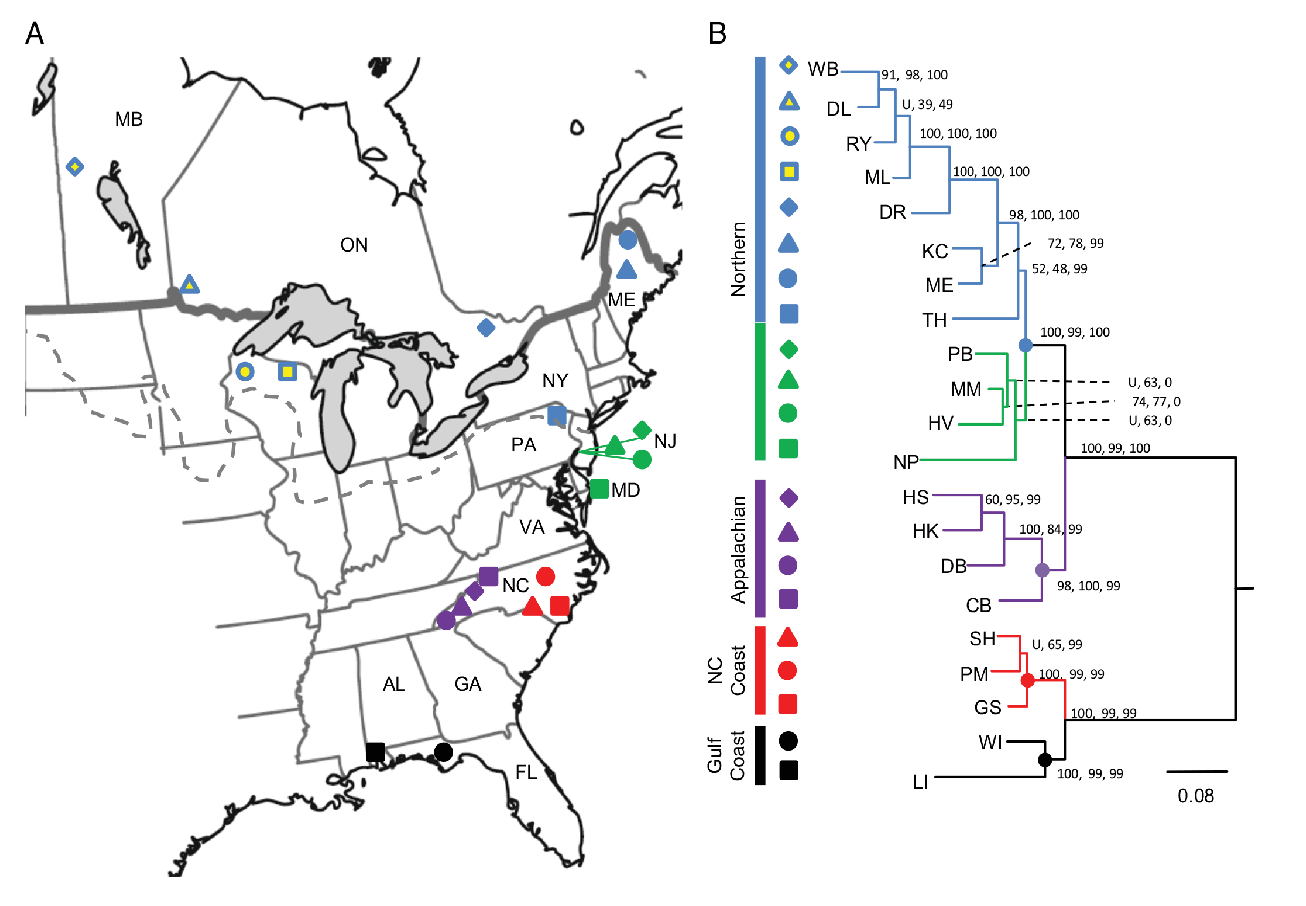
\includegraphics[height=0.9\textheight]{wyeomyia-RAD.eps}
\end{center}
}

\myslide{
  \heading{Nucleotide diversity: sample configuration at a homozygous site}

  \noindent Sample configuration
  \[
    (n_1, n_2, n_3, n_4) = \mbox{Number of }(A,C,G,T)\mbox{ in sample}
  \]
  \vfill
\[
P(n_1,n_2,n_3,n_4|\mbox{homozygous A},\epsilon)
=
{n \choose n_1}(1-\epsilon)^{n_1}\epsilon^{n-n_1}
\]
\vfill
\[
P(n_1,n_2,n_3,n_4|\mbox{homozygous},\epsilon)
=
\sum_{i=1}^4 \left(\frac{p_i^2}{\sum_{j=1}^4p_j^2}\right) 
{n \choose n_i}(1-\epsilon)^{n_i}\epsilon^{n-n_i}
\]
}

\myslide{
\heading{Nucleotide diversity: sample configuration at a heterozygous site}
\begin{eqnarray*}
  k_1 &=& \mbox{number of reads from chromosome 1} \\
  k_2 &=& \mbox{number of reads from chromosome 2} \\
P(k_1,k_2)
&=&
{n \choose k_1}\left(\frac{1}{2}\right)^{k_1}
               \left(\frac{1}{2}\right)^{k_2}
\\
&=&
{n \choose k_1}\left(\frac{1}{2}\right)^n
\end{eqnarray*}
}

\myslide{
\heading{Nucleotide diversity: sample configuration at a heterozygous site}
\vfill
{\footnotesize
  \begin{eqnarray*}
    x_i = \mbox{nucleotide on chromosome 1} \\
    x_j = \mbox{nucleotide on chromosome 2} \\
    \\
    \\
P(n_1,n_2,n_3,n_4|x_i,x_j,k_1,k_2) &=& \\
\sum_{l=1}^4\sum_{m=0}^{k_1}{k_1 \choose m}(1-\delta_{il})^m\delta_{il}^{k_1-m}
{k_2 \choose n_i-m}(1-\delta_{jl})^{n_1-m}\delta_{jl}^{k_2-(n_1-m)}
\end{eqnarray*}
}
where 
\[
\delta_{il} = \left\{\begin{array}{ll}
1-\epsilon & \mbox{if } i = l \\
\epsilon & \mbox{if } i \ne l \quad .
\end{array}
\right.
\]

}

\myslide{
\heading{Nucleotide diversity: sample configuration at a heterozygous site}
\[
P(n_1,n_2,n_3,n_4|x_i,x_j,\epsilon) =
P(n_1,n_2,n_3,n_4|x_i,x_j,k_1,k_2,\epsilon)P(k_1,k_2) \quad ,
\]
\vfill
{\footnotesize
\[
P(n_1,n_2,n_3,n_4|\mbox{heterozygous},\epsilon)
=
\sum_{i=1}^4\sum_{j\ne i}
\left(\frac{x_ix_j}{1-{\sum_{l=1}^4p_l^2}}\right) P(n_1,n_2,n_3,n_4|x_i,x_j,\epsilon) 
\]
}
}

\myslide{
\heading{Nucleotide diversity}
\[
\pi = \mbox{Probability that a site is heterozygous}
\]
\vfill
{\tiny
\[
P(n_1,n_2,n_3,n_4|\pi,\epsilon)
=
\pi P(n_1,n_2,n_3,n_4|\mbox{heterozygous},\epsilon)
+
(1-\pi)P(n_1,n_2,n_3,n_4|\mbox{homozygous},\epsilon) \quad .
\]
}
\vfill
\[
P(\mbox{data}|\pi,\epsilon) = \prod_{s=1}^S
P(n_1^{(s)},n_2^{(s)},n_3^{(s)},n_4^{(s)}|\pi,\epsilon)
\]
}

\myslide{
\heading{Nucleotide diversity}
\begin{center}
\begin{tabular}{lccc}
\hline\hline
Taxon & $4N_e\mu$ & $4N_e\mu$ (low coverage) & $\epsilon$ \\
\hline
{\it Cionia intestinalis} & 0.0111 & 0.012 & 0.00113 \\
{\it Daphnia pulex} & 0.0011 & 0.0012 & 0.00121 \\
\hline
\end{tabular}
\end{center}
}

\myslide{
\heading{PCA of population structure}
\begin{center}
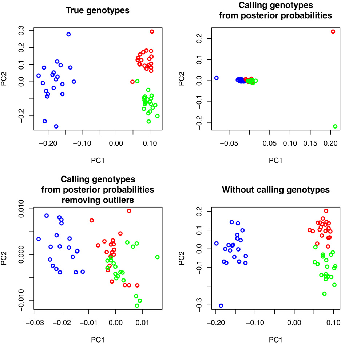
\includegraphics[height=0.9\textheight]{fumagalli-PCA.eps}
\end{center}
}

\myslide{
\heading{Population genomics in Great Britain}

Data
\begin{itemize}

\item 2039 individuals with four grandparents born within 80km of one
  another, effectively studying alleles sampled from grandparents
  (ca. 1885). 

\item 6209 samples from 10 countries in continental Europe.

\item Autosomal SNPs genotyped in both samples~(ca. 500K). 

\end{itemize}
\vfill
Results
\begin{itemize}

\item Average pairwise $F_{ST}$: 0.0007

\item Maximum pairwise $F_{ST}$: 0.003

\end{itemize}
}

\myslide{
\heading{Population genomics in Great Britain}

\begin{center}
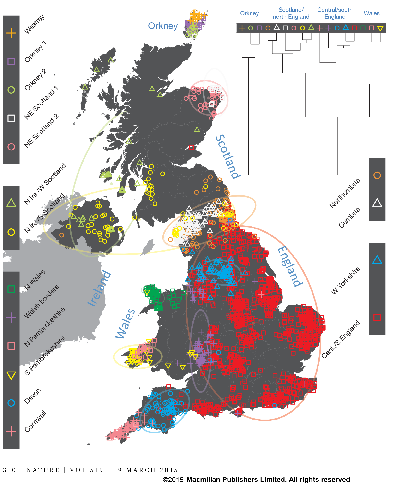
\includegraphics[height=0.9\textheight]{fine-structure-britain.eps}
\end{center}
}

\myslide{
\heading{Population genomics in Great Britain}

\begin{center}
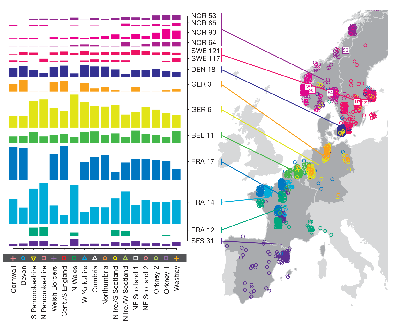
\includegraphics[height=0.9\textheight]{UK-Europe.eps}
\end{center}
}

\myslide{
  \heading{Polygenic inheritance}

\begin{center}
\resizebox{!}{0.9\textheight}{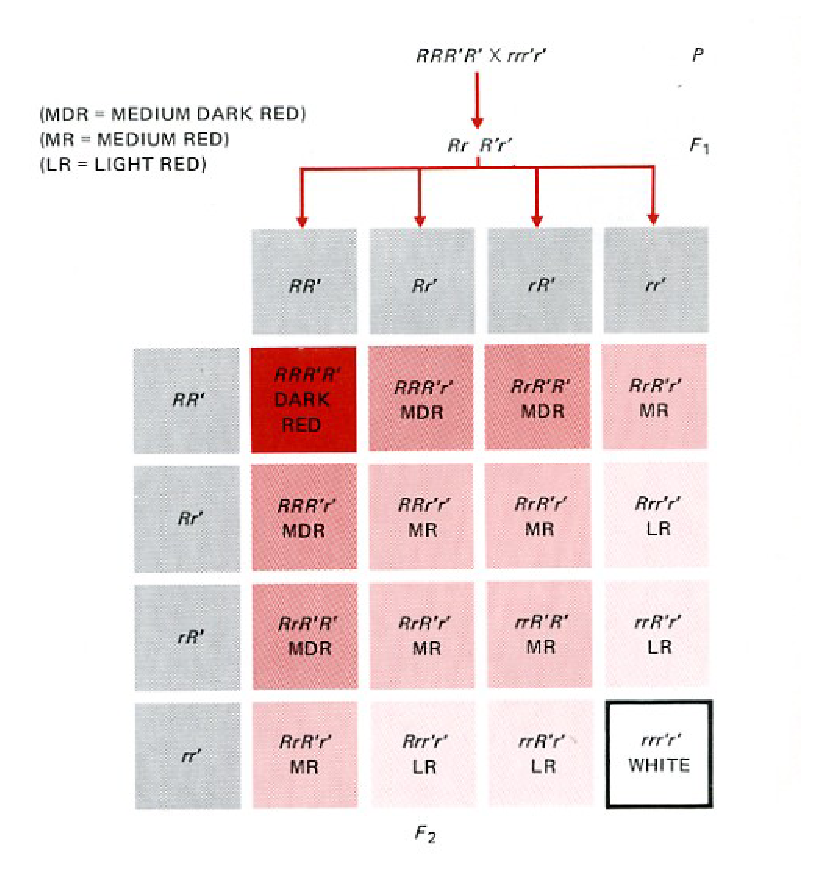
\includegraphics{Nilsson-Ehle.eps}}
\end{center}

}

\myslide{
\heading{Norm of reaction}
\begin{center}
\resizebox{!}{5cm}{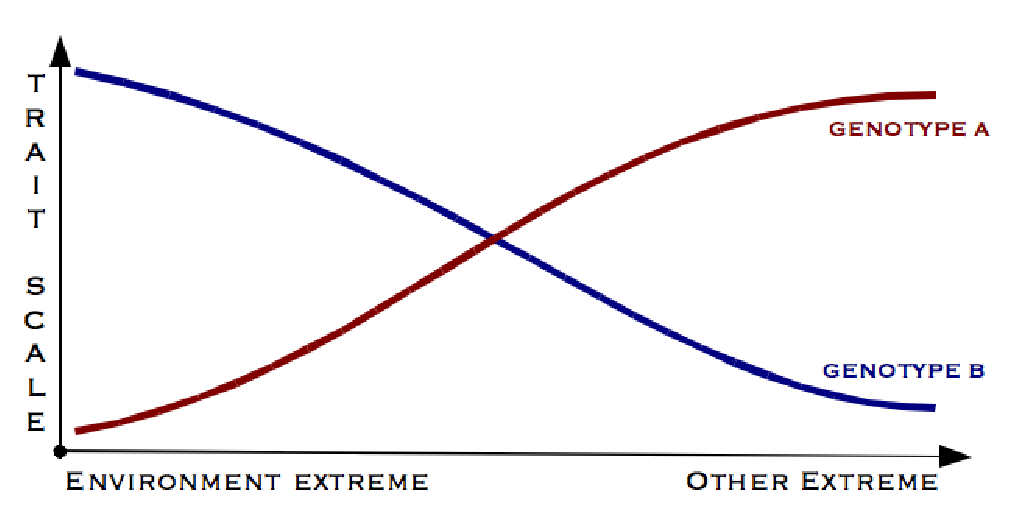
\includegraphics{Trait-scale-linear.eps}}
\end{center}
}

\myslide{
\heading{Where we're headed}
\[
\Var(P) = \Var(G) + \Var(E)
\]
\vfill
\[
h^2_n = \frac{\Var(A)}{\Var(P)}
\]
\vfill
\[
R = h^2_nS
\]
}

\myslide{
\begin{center}
\begin{tabular}{l|ccc}
\hline\hline
Genotype                 & $A_1A_1$    & $A_1A_2$ & $A_2A_2$ \\
\hline
Frequency                & $p^2$       & $2pq$    & $q^2$ \\
Genotypic value          & $x_{11}$    & $x_{12}$ & $x_{22}$ \\
Additive genotypic value & $2\alpha_1$ & $\alpha_1 + \alpha_2$ 
                                                  & $2\alpha_2$ \\
\hline
\end{tabular}
\end{center}
}

\myslide{
\heading{Genotypic value}
\begin{center}
\resizebox{!}{7cm}{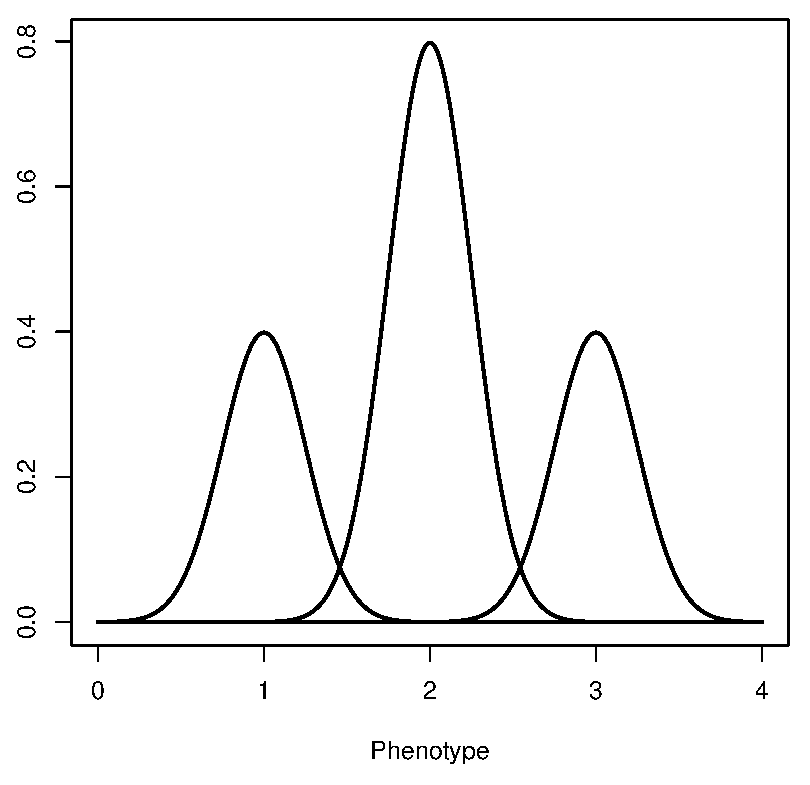
\includegraphics{genotypic-value.eps}}
\end{center}
}

\myslide{
\[
a = p^2[x_{11}-2\alpha_1]^2
       + 2pq[x_{12}-(\alpha_1+\alpha_2)]^2
       + q^2[x_{22}-2\alpha_2]^2 \quad .
\]
\vfill
\begin{eqnarray*}
\frac{\partial a}{\partial{\alpha_1}} &=& p^2\{2[x_{11} - 2\alpha_1][-2]\}
                     + 2pq\{2[x_{12} - (\alpha_1+\alpha_2)][-1]\} \\
                  &=& -4p^2[x_{11} - 2\alpha_1]
                     -4pq[x_{12} - (\alpha_1+\alpha_2)] \\
\frac{\partial a}{\partial{\alpha_2}} &=& q^2\{2[x_{22} - 2\alpha_2][-2]\}
                     + 2pq\{2[x_{12} - (\alpha_1+\alpha_2)][-1]\} \\
                  &=& -4q^2[x_{22} - 2\alpha_2]
                     -4pq[x_{12} - (\alpha_1+\alpha_2)] 
\end{eqnarray*}
}

\myslide{
\begin{eqnarray*}
p^2(x_{11} - 2\alpha_1) + pq(x_{12} - \alpha_1 - \alpha_2) &=& 0
  \nonumber \\
q^2(x_{22} - 2\alpha_2) + pq(x_{12} - \alpha_1 - \alpha_2) &=& 0
\end{eqnarray*}
\vfill
\[
[p^2x_{11} + 2pqx_{12} + q^2x_{22}] -
   [p^2(2\alpha_1) + 2pq(\alpha_1 + \alpha_2) + q^2(2\alpha_2)] = 0
\]
\vfill
\begin{eqnarray*}
{\bar x} &=& 2p^2\alpha_1 + 2pq(\alpha_1 + \alpha_2)
                        +2q^2\alpha_2 \nonumber \\
                     &=& 2p\alpha_1(p+q) + 2q\alpha_2(p+q) \nonumber \\
                     &=& 2(p\alpha_1 + q\alpha_2)
\end{eqnarray*}
}

\myslide{
\begin{eqnarray*}
p^2(x_{11} - 2\alpha_1) + pq(x_{12} - \alpha_1 - \alpha_2) &=& 0
  \nonumber \\
q^2(x_{22} - 2\alpha_2) + pq(x_{12} - \alpha_1 - \alpha_2) &=& 0
\end{eqnarray*}
\vfil
\begin{eqnarray*}
p(x_{11} - 2\alpha_1) + q(x_{12} - \alpha_1 - \alpha_2) &=& 0 \\
q(x_{22} - 2\alpha_2) + p(x_{12} - \alpha_1 - \alpha_2) &=& 0 
\end{eqnarray*}
\begin{eqnarray*}
px_{11} + qx_{12} &=& 2p\alpha_1 + q\alpha_1 + q\alpha_2 \\
 &=& \alpha_1(p + q) + p\alpha_1 + q\alpha_2 \\
 &=& \alpha_1 + p\alpha_1 + q\alpha_2 \\
 &=& \alpha_1 + {\bar x}/2 \\
\alpha_1 &=& px_{11} + qx_{12} - {\bar x}/2 \\
\alpha_2 &=& px_{12} + qx_{22} - {\bar x}/2
\end{eqnarray*}
}

\myslide{
\begin{eqnarray*}
V_g &=&\ p^2[x_{11} - {\bar x}]^2 + 2pq[x_{12} - {\bar x}]^2
     + q^2[x_{22} - {\bar x}]^2 \label{eq:v-g} \\
    &=&\ p^2[x_{11} - 2\alpha_1 + 2\alpha_1 - {\bar x}]^2
     + 2pq[x_{12} - (\alpha_1 + \alpha_2) + (\alpha_1 + \alpha_2)
                - {\bar x}]^2 \nonumber \\
     &&\ \ + q^2[x_{22} - 2\alpha_2 + 2\alpha_2 - {\bar x}]^2
     \nonumber \\
    &=&\ p^2[x_{11} - 2\alpha_1]^2 + 2pq[x_{12} - (\alpha_1+\alpha_2)]^2
       + q^2[x_{22} - 2\alpha_2]^2 \nonumber \\
     &&\ + p^2[2\alpha_1 - {\bar x}]^2 + 2pq[(\alpha_1 + \alpha_2) - {\bar x}]^2
       + q^2[2\alpha_2 - {\bar x}]^2 \nonumber \\
     &&\ + p^2[2(x_{11} - 2\alpha_1)(2\alpha_1 - {\bar x})] \\
     &&\ +2pq[2(x_{12} - \{\alpha_1+\alpha_2\})(\{\alpha_1+\alpha_2\} -
     {\bar x})] \nonumber \\
     &&\ +q^2[2(x_{22} - 2\alpha_2)(2\alpha_2 - {\bar x})] \quad .
\end{eqnarray*}
}

\myslide{
\begin{center}
\begin{tabular}{l|ccc}
\hline\hline
Genotype        & $A_1A_1$ & $A_1A_2$ & $A_2A_2$ \\
Genotypic value &  0       & 1        & 2 \\
\hline
\end{tabular}
\end{center}
\vfill
For $p=0.4$
\begin{eqnarray*}
{\bar x} &=& (0.4)^2(0) + 2(0.4)(0.6)(1) + (0.6)^2(2) \\
                    &=& 1.20 \\
\\
\alpha_1 &=& (0.4)(0) + (0.6)(1) - (1.20)/2 \\
         &=& 0.0 \\
\alpha_2 &=& (0.4)(1) + (0.6)(2) - (1.20)/2 \\
         &=& 1.0
\end{eqnarray*}
}

\myslide{
\begin{eqnarray*}
V_g &=& (0.4)^2(0-1.20)^2 + 2(0.4)(0.6)(1-1.20)^2 + (0.6)^2(2-1.20)^2 \\
    &=& 0.48 \\
V_a &=& (0.4)^2[2(0.0)-1.20]^2 + 2(0.4)(0.6)[(0.0+1.0)-1.20]^2 \\
    &&   + (0.6)^2[2(1.0)-1.20]^2 \\
    &=& 0.48 \\
V_d &=& (0.4)^2[0 - 2(0.0)]^2 + 2(0.4)(0.6)[1 - (0.0+1.0)]^2 \\
    &&   + (0.6)^2[2 - 2(1.0)]^2 \\
    &=& 0.00
\end{eqnarray*}
}

\myslide{
\begin{center}
\begin{tabular}{l|ccc}
\hline\hline
Genotype        & $A_1A_1$ & $A_1A_2$ & $A_2A_2$ \\
Genotypic value & 0        & 0.8      & 2 \\
\hline
\end{tabular}
\end{center}
\vfill
For $p=0.4$
\begin{eqnarray*}
{\bar x} &=& (0.4)^2(0) + 2(0.4)(0.6)(0.8) + (0.6)^2(2) \\
                    &=& 1.104 \\
\\
\alpha_1 &=& (0.4)(0) + (0.6)(0.8) - (1.104)/2 \\
         &=& -0.072 \\
\alpha_2 &=& (0.4)(0.8) + (0.6)(2) - (1.104)/2 \\
         &=& 0.968 \\
\end{eqnarray*}
}

\myslide{
\begin{eqnarray*}
V_g &=& (0.4)^2(0-1.104)^2 + 2(0.4)(0.6)(0.8-1.104)^2 + (0.6)^2(2-1.104)^2 \\
    &=& 0.5284 \\
V_a &=& (0.4)^2[2(-0.072)-1.104]^2 + 2(0.4)(0.6)[(-0.072+0.968)-1.104]^2 \\
       &&+ (0.6)^2[2(0.968)-1.104]^2 \\
    &=& 0.5192 \\
V_d &=& (0.4)^2[0 - 2(-0.072)]^2 + 2(0.4)(0.6)[0.8 - (-0.072+0.968)]^2 \\
       &&+ (0.6)^2[2 - 2(0.968)]^2 \\
    &=& 0.0092
\end{eqnarray*}
}

\myslide{
\[
\Cov(X,Y) = \sum p_{xy}(x - \mu_x)(y - \mu_y)
\]
}

\myslide{
\begin{center}
\begin{tabular}{c|c|ccc}
\hline\hline
Maternal &           & \multicolumn{3}{c}{Offspring genotype} \\
genotype & Frequency & $A_1A_1$      & $A_1A_2$      & $A_2A_2$ \\
\hline
$A_1A_1$ & $p^2$     & $p$           & q             & 0 \\
$A_1A_2$ & $2pq$     & $\frac{p}{2}$ & $\frac{1}{2}$ & $\frac{q}{2}$ \\
$A_2A_2$ & $q^2$     & 0             & p             & q \\
\hline
\end{tabular}
\end{center}
\vfill
\begin{eqnarray*}
\Cov(S_1,S_2) &=& p^2[p^2(x_{11} - {\bar x})^2 + 2pq(x_{11} - {\bar x})
                                                (x_{12} - {\bar x})
                                           + q^2(x_{12} - {\bar x})^2] \\
             &&+ 2pq[{1 \over 4}p^2(x_{11} - {\bar x})^2
                  + {1 \over 2}p(x_{11} - {\bar x})(x_{12} - {\bar x}) \\
             &&   + {1 \over 2}pq(x_{11} - {\bar x})(x_{22} - {\bar
                    x}) 
                  + {1 \over 4}(x_{12} - {\bar x})^2
                  \\
             &&   + {1 \over 2}q(x_{12} - {\bar x})(x_{22} - {\bar x})
                  + {1 \over 4}q^2(x_{22} - {\bar x})^2] \\
             &&+ q^2[p^2(x_{12} - {\bar x})^2 + 2pq(x_{12} - {\bar x})
                                                 + q^2(x_{22} - {\bar
                                                x})] 
\end{eqnarray*}
}

\myslide{
TAMO
\[
\Cov(S_1, S_2) = \left({1 \over 4}\right)V_a
\]
}

\myslide{
\begin{center}
\begin{tabular}{l|ccc}
\hline\hline
Genotype  & $A_1A_1$ & $A_1A_2$ & $A_2A_2$ \\
Phenotype & 0        & 0.8      & 2 \\
\hline
\end{tabular}
\end{center}
\vfill
\begin{center}
\begin{tabular}{c|c|ccc}
\hline\hline
Maternal &           & \multicolumn{3}{c}{Offspring genotype} \\
genotype & Frequency & $A_1A_1$ & $A_1A_2$ & $A_2A_2$ \\
\hline
$A_1A_1$ & 0.16      & 0.4      & 0.6      & 0.0 \\
$A_1A_2$ & 0.48      & 0.2      & 0.5      & 0.3 \\
$A_2A_2$ & 0.36      & 0.0      & 0.4      & 0.6 \\
\hline
\end{tabular}
\end{center}
\vfill
\begin{eqnarray*}
\Cov(S_1,S_2) &=& 0.1298 \\
             &=& \left(\frac{1}{4}\right)0.5192
\end{eqnarray*}
}

\myslide{
\begin{eqnarray*}
b_{P \rightarrow O}
&=& \frac{\Cov_{PO}}{\Var(P)} \\
&=& {\left({1 \over 2}\right)V_a \over V_p} \\
&=& \left({1 \over 2}\right)h^2_N 
\end{eqnarray*}
}

\myslide{
\begin{eqnarray*}
\Var(MP) &=& \Var\left(\frac{M+F}{2}\right) \\
                  &=& \frac{1}{4} \Var(M+F) \\
                  &=& \frac{1}{4} \left(Var(M) + Var(F)\right) \\
                  &=& \frac{1}{4} \left(2V_p\right) \\
                  &=& \frac{1}{2} V_p \\
b_{MP\rightarrow O} &=& \frac{\left(\frac{1}{2}\right)V_a} 
                           {\left(\frac{1}{2}\right)V_p} \\
                  &=& h^2_N
\end{eqnarray*}
}

\myslide{
\begin{center}
\begin{tabular}{l|ccc}
\hline\hline
        &      &             & Composition of \\
Source  & d.f. & Mean square & mean square \\
\hline
Among sires             & $s-1$     & $MS_S$ 
                        & $\sigma^2_W + k\sigma^2_D + dk\sigma^2_s$ \\
Among dams              & $s(d-1)$  & $MS_D$
                        & $\sigma^2_W + k\sigma^2_D$ \\
\hskip 1em (within sires) \\
Within progenies        & $sd(k-1)$ & $MS_W$
                        & $\sigma^2_W$\\
\hline
\multicolumn{4}{l}{$s = \hbox{number of sires}$} \\
\multicolumn{4}{l}{$d = \hbox{number of dams per sire}$} \\
\multicolumn{4}{l}{$k = \hbox{number of offspring per dam}$} 
\end{tabular}
\end{center}
}

\myslide{
\small
\begin{eqnarray*}
\sigma^2_S &=& \Cov_{HS} \\
           &=& \left(\frac{1}{4}\right)V_a
\end{eqnarray*}
\vfill
\begin{eqnarray*}
\sigma^2_W &=& V_p - \Cov_{FS} \\
 &=& V_a + V_d + V_e - \left[\left(\frac{1}{2}\right)V_a + 
                            \left(\frac{1}{4}\right)V_d
                      \right] \\
 &=& \left(\frac{1}{2}\right)V_a 
    + \left({3 \over 4}\right)V_d
    + V_e
\end{eqnarray*}
\vfill
\begin{eqnarray*}
\sigma^2_D &=& \Cov_{FS} - \Cov_{HS} \\
           &=& \left[
              \left(\frac{1}{2}\right)V_a + \left(\frac{1}{4}\right)V_d 
              \right]
              - \left(\frac{1}{4}\right)V_a \\
           &=& \left(\frac{1}{4}\right)V_a +
           \left(\frac{1}{4}\right)V_d
\end{eqnarray*}
}

\myslide{
\begin{eqnarray*}
V_a &=& 4\sigma^2_S \\
V_d &=& 4(\sigma^2_D - \sigma^2_S) \\
V_e &=& \sigma^2_W - 3\sigma^2_D + \sigma^2_S \quad .
\end{eqnarray*}
}

\myslide{
\begin{center}
\begin{tabular}{l|ccc}
\hline\hline
        &      &             & Composition of \\
Source  & d.f. & Mean square & mean square \\
\hline
Among sires             & 70 & 17.10 
                        & $\sigma^2_W + k'\sigma^2_D + dk'\sigma^2_s$ \\
Among dams              & 118 & 10.79
                        & $\sigma^2_W + k\sigma^2_D$ \\
\hskip 1em (within sires) \\
Within progenies        & 527 & 2.19
                        & $\sigma^2_W$ \\
\hline
\multicolumn{4}{l}{$d = 2.33$} \\
\multicolumn{4}{l}{$k = 3.48$} \\
\multicolumn{4}{l}{$k' = 4.16$} \\
\end{tabular}
\end{center}
}

\myslide{
\small
\begin{eqnarray*}
\sigma^2_W &=& MS_W \\
           &=& 2.19 \\
\sigma^2_D &=& \left({1 \over k}\right)(MS_D - \sigma^2_W) \\
           &=& 2.47 \\
\sigma^2_S &=& \left({1 \over dk'}\right)(MS_S - \sigma^2_W 
                    - k'\sigma^2_D) \\
           &=& 0.48
\end{eqnarray*}
\vfill
\begin{eqnarray*}
V_p &=& 5.14 \\
V_a &=& 1.92 \\
V_d + V_e &=& 3.22 \\
V_d &=& (0.00\hbox{---}1.64) \\
V_e &=& (1.58\hbox{---}3.22) \\
h^2_N &=& 0.37
\end{eqnarray*}
}

\end{document}
